\documentclass[letterpaper,11pt]{article}

\usepackage{graphicx}
\usepackage{multicol}
\usepackage{fullpage}
\usepackage{csquotes}
\usepackage[margin=0.5in,letterpaper]{geometry}
\setlength{\footskip}{15pt}
\usepackage{floatflt}
\usepackage{xspace}
\linespread{0.95}
\def\degC{$^{\circ}$C }
\def\degf{$^{\circ}$F }
\def\vol #1 {{\bf #1}, $\;\;$}
\def\refer{\par\noindent\hangindent\parindent\hangafter1}


\title{\vspace{-2.0cm}Herzmann Family Christmas Letter 2018}
\author{Daryl Herzmann${}^1$, Elizabeth Herzmann${}^1$, Margaret 
Herzmann${}^2$,\\
Robert Herzmann${}^3$, AND Charlotte Herzmann${}^4$ \\
\it{${}^1$ Caretakers},
\it{${}^2$ Senior Child},
\it{${}^3$ Little Stinker},
\it{${}^4$ Fussing Monster}}
\date{16 December 2018}

\makeatletter
\newenvironment{tablehere}
  {\def\@captype{table}}
  {}

\newenvironment{figurehere}
  {\def\@captype{figure}}
  {}
\makeatother

\newcommand{\Line}[0]{%
  \rule{0cm}{0cm}\\\hrule\rule{0cm}{0cm}%
}

%\addtolength{\textheight}{1.5in}

\begin{document}
\maketitle
\vspace{-0.75cm}
\begin{abstract}
Attrition prevailed and we arrive at the end of another year. This year's
dossier will strive to not violate state gaming laws nor commit mail fraud. It
turns out that giving away Amazon.com gift cards via a Christmas Letter may not
be the best means to boost readership.  Much has happened in the past year and
you are about to be informed of it without any possible direct financial gain.
\end{abstract}

\vspace{-0.5cm}
\Line
%\vspace{-0.5cm}

\begin{multicols}{2}

\section{Introduction} 

The size of our family was not altered this year and comprises Daryl
\enquote{Daryl} (40), Elizabeth \enquote{Liz} (age redacted),
Margaret \enquote{Miss Maggie} (5), Robert \enquote{Ro-Ro} (4), Charlotte
 \enquote{Charly} (1), and one cat with a dog's name of Snoopy (10).  The near
 term probability forecast for increasing the family size is near zero with
 Figure 1 showing the current stretch of non-pregnancy achieved.  

\subsection{Housing}

No changes have been made with our housing arrangement. 2019 will mark the
'seven year itch' predicted by our real estate agent for when we would desire
to change housing. Out of spite for that prediction, we will not be moving.

\subsection{Conveyances}

Herzmann et al (2017) boasted that no new car, read minivan, would be necessary
for Daryl, but one day Mr Robert inquired if he should hide in his seat when
we drove past a cop car as his present car seat was not the right size. A few
weeks later a new Honda Pilot, read minivan, was purchased.  Mr Robert can
worry about avoiding the police later in life now.

We loaded up the three kids and took Liz's minivan on a spring break trip to
the Big D and I do mean Dallas. The kids did remarkably well for the many
hours of riding in the car and enjoyed visiting their Great Grandmother and
cousins there.  We stopped at Legoland in Kansas City, which they had great
fun at.

\subsection{Employment}
Daryl remains employed by Iowa State University. Sadly his friend and supervisor
for the past 16 years died suddenly from a stroke on the same date that Daryl's
father died eight years ago (14 November). Daryl has been adopted by another
faculty member at ISU and should have funding to keep going.

\begin{figurehere}
 \centering   
 \resizebox{.95\columnwidth}{!}{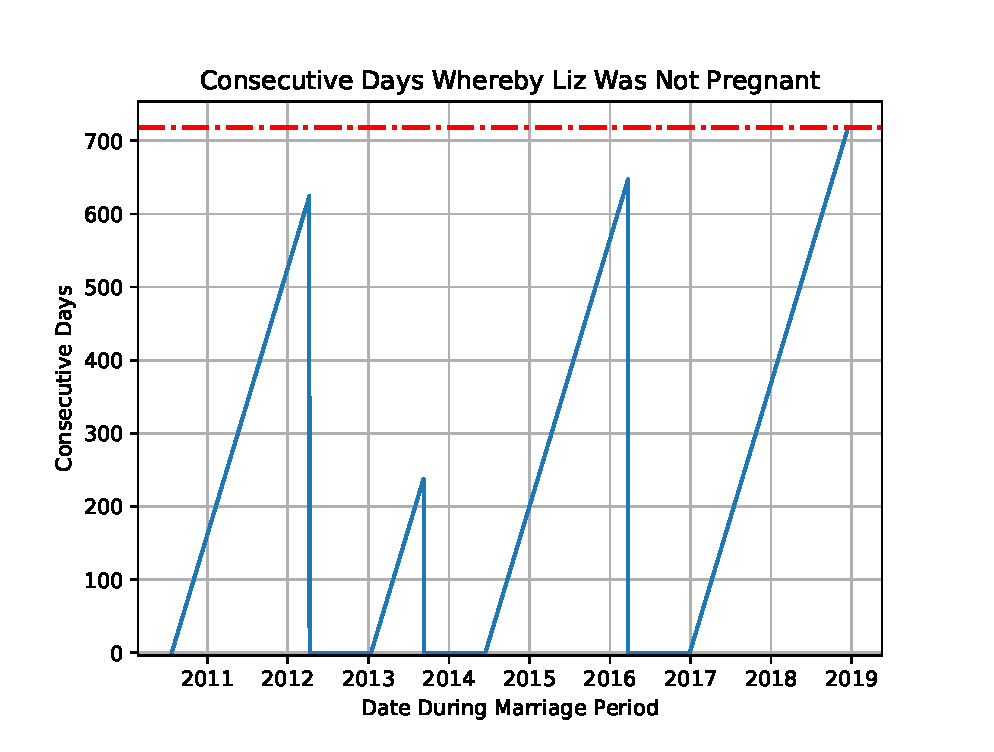
\includegraphics[angle=0]{plots/prego.eps}}
 \caption{Currently at marriage record duration for not being pregnant.}
\end{figurehere}

After a wonderful 8 years teaching in Johnston, Liz was able to land a
science teaching position in our hometown of Ankeny this school year. She is working
with 8th graders at Southview Middle School.  The new commute of 5 minutes
has proven beneficial given our children's ever expanding list of
activities.  Biking to work was seriously considered, but in the end she
decided to give it a year to settle in first.

The other 60\% of our family is ignorant of minimum wage and happily does odd
jobs for shiny pennies.  Miss Maggie thought briefly that a dollar could be
worth 100 pennies, but the parents squashed that rebellion.

\section{Miss Charlotte}

Miss Charlotte's development has been fun to observe.  She presently knows many
words, but has yet to conjugate a sentence.  She was recently evicted from her
crib and into a standard issue twin bed.  Her wakeup routine is
to collect up all her blankeys, stuffed animals, and binkeys before heading
downstairs for breakfast.  Her stuffed animals are then arranged on the table
as shown by Figure 2.

\bigskip

\begin{figurehere}
 \centering   
 \resizebox{.95\columnwidth}{!}{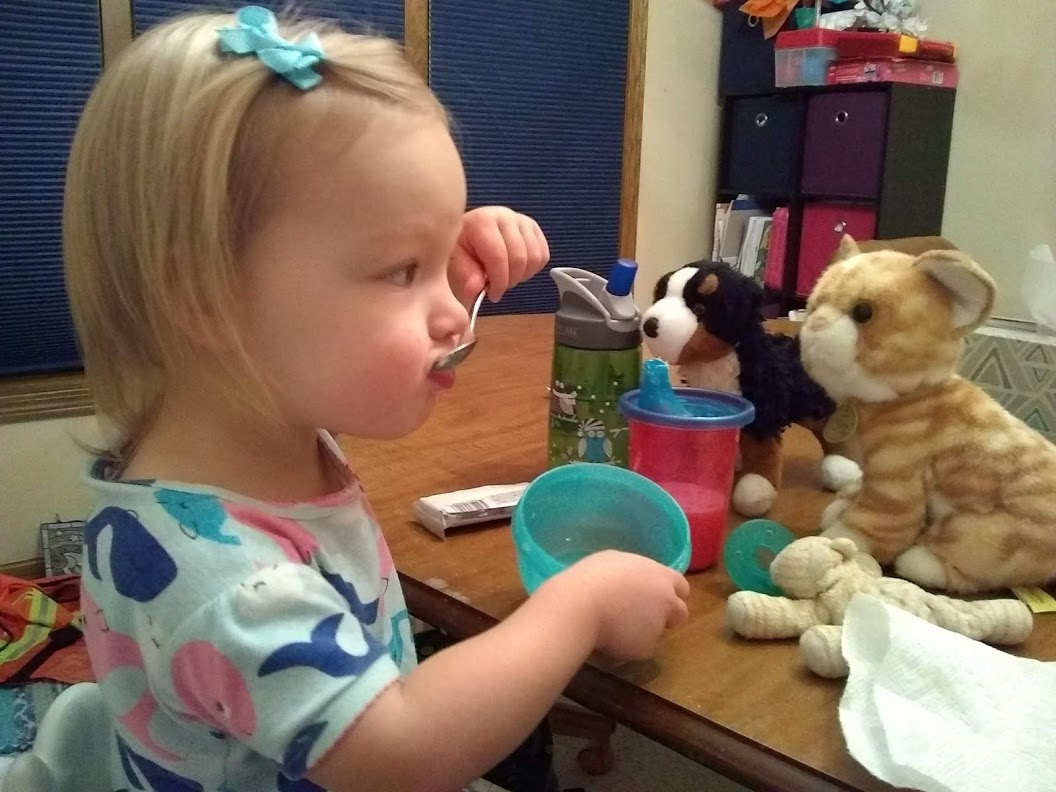
\includegraphics[angle=0]{plots/left.eps}}
 \caption{Charlotte eating breakfast with her left hand.}
\end{figurehere}

\bigskip

Miss Charlotte loves to wrestle with anybody in the family willing and is already
roughing up Mr Robert more than he likes.  She is still a picky eater and prefers
to consume pancakes two at a time, one for each hand.

\section{Mr Robert}

Mr Robert is handful bundle of joy.  While his age is on the fence to be sent
to kindergarten in the fall, we are currently leaning toward enrolling him and
see what transpires. Mr Robert loves to play, be loud, and complain about his sisters,
parents, and the world in general being unfair to him.  He has breathtaking moments of
lucid deduction though, which are cherished memories for us.  For instance, he will
scream, while not wanting to go to bed, that if he stays up screaming that he will 
wake up grumpy tomorrow. He also seems to have an intrinsic understanding of
logistics and will make observations regarding inefficiencies with parental
workflows.

\section{Miss Maggie}

Miss Maggie is enjoying her first year of school at kindergarten and seems to be
a model student so far.  We were able to get her into our nearby elementary school,
which is a quick walk from our house.  She has surprised us with how quickly she
has picked up reading and doing math tasks.  Her favorite books include
\enquote{Fancy Nancy}, \enquote{WellieWishers}\texttrademark, and
\enquote{Berenstain Bears}.

\section{Summary}

We hoped you enjoyed reading this article, which was mailed with great care
as shown by Figure 3.  While tiring, life in our household is fun and full of
love.  The three children are such wonderful blessings and often remind us of
how fortunate we are. 

\bigskip
\begin{figurehere}
 \centering   
 \resizebox{.95\columnwidth}{!}{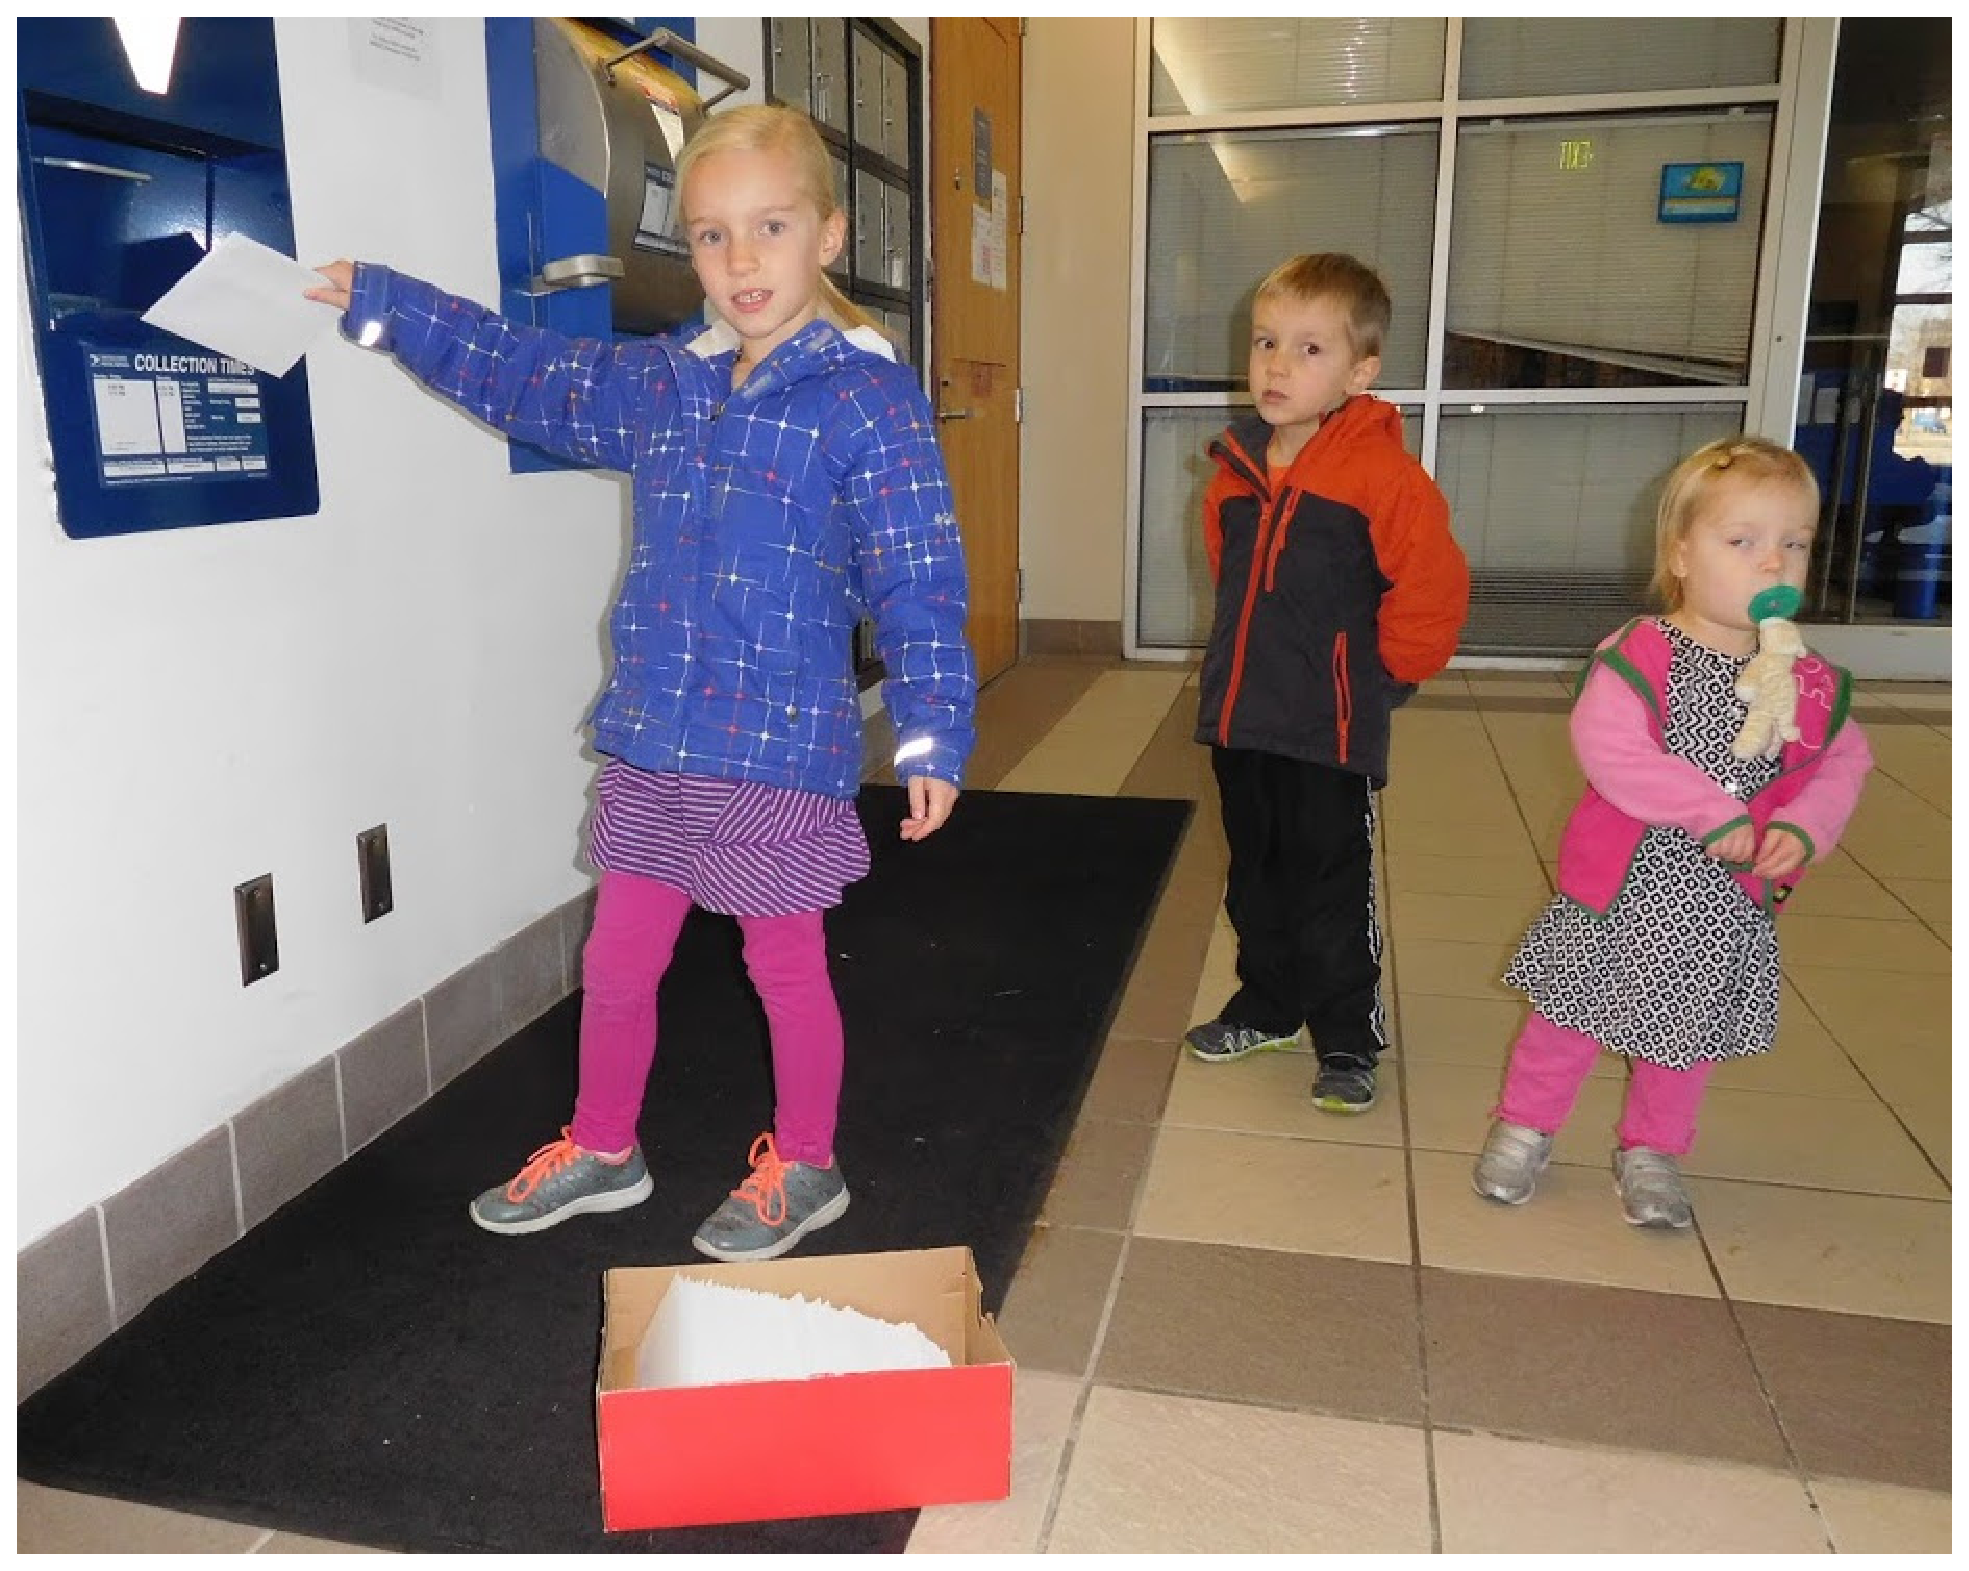
\includegraphics[angle=0]{plots/mail.eps}}
 \caption{The children delivering this year's letter to our local Amazon owned
 US Post Office. Miss Maggie thought it would be fun to place one letter at 
 a time into the mail box.}
\end{figurehere}

\bigskip
  \emph{Acknowledgments} Our family wishes to thank you for the generous 
support, prayers, cards, gifts, and visits you have provided us in the past
year. With your continued support, this letter will be produced again
next year. Please note that the format chosen for this
correspondence was completely Daryl's idea and execution. Liz had marginal
editorial control. Full \LaTeX\xspace source can be found on Daryl's Github
page.

\section{References}

\refer Github, 2018: https://github.com/akrherz/me , visited 15 Dec 2018.
\refer Herzmann, Daryl E., et al. Herzmann Family Christmas Letter 2017. 

\end{multicols}

\end{document}

